% Don't modify this section unless you know what you're doing!
\documentclass[letterpaper,12pt]{article}
\usepackage{float}
\usepackage[spanish]{babel}
\selectlanguage{spanish}
\usepackage[utf8]{inputenc}
\usepackage{tabularx} % extra features for tabular environment
\usepackage{amsmath}  % improve math presentation
\usepackage{graphicx, wrapfig, subcaption, setspace, booktabs}
\usepackage{graphicx} % takes care of graphic including machinery

\usepackage[margin=1in,letterpaper]{geometry} % decreases margins
\usepackage{cite} % takes care of citations
\usepackage[final]{hyperref} % adds hyper links inside the generated pdf file
\usepackage{amsmath}
\usepackage{amssymb}
\usepackage{enumerate}
\usepackage{url}
\hypersetup{
	colorlinks=true,       % false: boxed links; true: colored links
	linkcolor=blue,        % color of internal links
	citecolor=blue,        % color of links to bibliography
	filecolor=magenta,     % color of file links
	urlcolor=blue         
}
%++++++++++++++++++++++++++++++++++++++++


\begin{document}

\title{Reporte de la actividad 7}
\author{Daniela Olmos Velderrain\\Grupo 3}
\date{24 de marzo de 2019}

\maketitle

\section{Introducción}
    En esta actividad analizamos los datos en una estación meteorológica de un campo de nogal para observar las correlaciones entre distintos parámetros medidos. Se comparó el uso de las bibliotecas SeaBorn y Matplotlib para la elaboración de gráficos, y también se graficaron las variables que mostraban un alto índice de correlación. 
    
\section{Desarrollo}
\subsection{Marco teórico}
\subsubsection{Correlación}
Se considera que dos variables cuantitativas están correlacionadas cuando los valores de una de ellas varían sistemáticamente con respecto a los valores homónimos de la otra: si tenemos dos variables (A y B) existe correlación entre ellas si al disminuir los valores de A lo hacen también los de B y viceversa.

\subsubsection{Heat Map}
Un heatmap o mapa de calor es una representación gráfica que utiliza tonos de color de diferente intensidad para indicar las zonas con mayor incidencia. En esta actividad el uso de mapas de calor será útil para ubicar las variables con mayor correlación del data frame.


\subsection{Metodología} 
Para comenzar a trabajar con el archivo, primero fue necesario descargar librerías para el análisis de datos y visualización:

\begin{verbatim}
import pandas as pd
import numpy as np
import matplotlib.pyplot as plt
import seaborn as sns
import math
\end{verbatim}

Como el archivo a leer contenía caracteres especiales que no podía reconocer la librería de Pandas, utilizamos el lector de python:

\begin{verbatim}
    df = pd.DataFrame( pd.read_csv("meteo-nogal-09.csv", engine="python" ) )
\end{verbatim}

El documento contaba con varias columnas nombradas "unnamed" que no contenían datos relevantes, así que las eliminamos para quedarnos con un data frame más pequeño:

\begin{verbatim}
    df=df.drop(df.columns[df.columns.str.contains('unnamed:',case = False)],axis = 1)
\end{verbatim}
 
 Como el archivo no contaba con una variable de datetime, la creamos a partir de dos columnas que contenían fechas y horas: 
 
\begin{verbatim}
  df["FECHA"] = df["DATE"] + " "+ df["TIME"]
\end{verbatim}

Convertimos las variables object a float64 para poder operar con los datos de forma numérica:

\begin{verbatim}
    df[df.columns[0:14]] = df[df.columns[0:14]].apply(pd.to_numeric, errors='coerce')
\end{verbatim}

Empleamos la función $corr$ para encontrar las correlaciones entre las variables:

\begin{verbatim}
df_corr = df.corr(method='pearson', min_periods=1)
\end{verbatim}

Con el data frame de las correlaciones creamos dos gráficas del tipo heatmap, una mediante la bilbioteca Seaborn y otra mediante Matplotlib.

Por último, observamos las correlaciones cuyo valor absoluto era mayor a 0.5 y las graficamos. 

\subsection{Resultados}
A continuación se muestran las gráficas de heatmap elaboradas con Seaborn y Matplotlib:

\begin{center}
	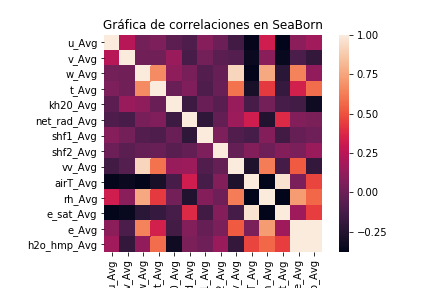
\includegraphics[height=5cm]{correlaciones_sns.png}\hspace*{\fill}
	\label{graf1}
   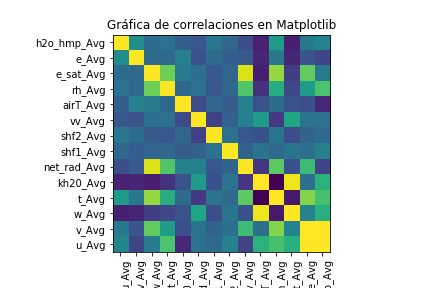
\includegraphics[height=5cm]{correlaciones_mpltlib.png}
    \label{graf2}
\end{center}

Aunque las dos son similares en apariencia, el diagrama de Seaborn cuenta con una barra que indica la correlación correspondiente a cada color, lo cual no se pudo lograr en Matplotlib.

Las correlaciones mayores a 0.5 fueron 12 en total. A continuación se mostrarán dos casos, uno en que la correlación es muy cercana a 0.5 y otro en que es muy cercana a 1.

\begin{center}
	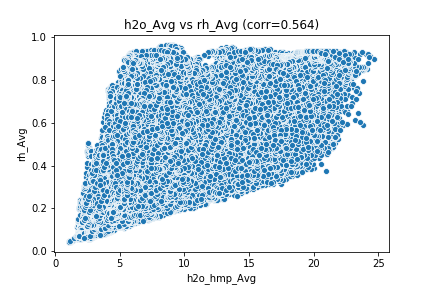
\includegraphics[height=5cm]{corr12.png}\hspace*{\fill}
	\label{graf3}
   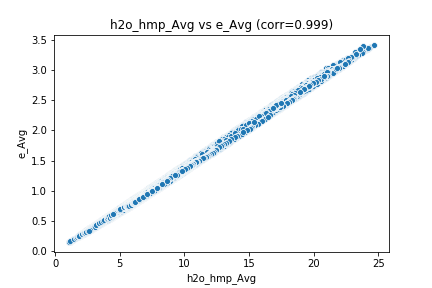
\includegraphics[height=5cm]{corr11.png}
    \label{graf4}
\end{center}

\section{Conclusiones}
Al comparar el uso de ambas bibliotecas al momento de graficar, notamos inmediatamente la gran facilidad que tiene SeaBorn en comparación a Matplotlib, ya que se ocuparon muchas más líneas de código para elaborar el heatmap en Matplotlib, y este no contenía la barra lateral que proporciona SeaBorn.

En cuanto a las gráficas de correlaciones, se puede observar a simple vista que a medida que la correlación se aproxima más a 1 la relación entre las variables es más coherente, mientras que al alejarse de este valor las variables parecen no tener relación entre sí. 

\section*{Bibliografía}
\begin{itemize}

\item \\Correlación. Recuperado el 24 de marzo de 2019 desde \\https://es.wikipedia.org/wiki/Correlaci\%C3\%B3n
\\

\item \\Mapa de Calor. Recuperado el 24 de marzo de 2019 desde \\https://www.oleoshop.com/blog/mapa-de-calor-que-es
\end{itemize}


\end{document}
